%!TEX root = mb.tex

\section{Overview}\label{sec:overview}

In this section, we present \sys's architecture, the threat model and applications supported.

\subsection{Aplomb and NEF architecture}

We recall the system setup in Aplomb and NEF setup, illustrated in Fig.~\ref{fig:sys-overview}. 
There are three parties: enterprise(s), the cloud running the middlebox, and an external site providing
some service. 
The enterprise runs a gateway (GW) which sends traffic to a middlebox (MB) running in the cloud.

There are two setups. The first setup occus when the enteprise communicates with an external site.  In this case, we have setup as in Fig.~\ref{fig:model1}.
The traffic from a client inside the enteprise passes the gateway on the way out of the enterprise. The gateway redirects this traffic to the middlebox in the cloud.
After performing various middlebox processing, MB returns the traffic to the gateway. The gateway finally sends the traffic to the external site. 
The answer from the external site follows the reverse direction of the
request.


The second setup occurs when the traffic is sent between two enterprises as in Fig.~\ref{fig:model2}. This allows for a more optimized and faster layout. Each enterprise has it's own gateway.
Traffic from a client in enterprise 1 passes through the gateway of this enterprise which redirects it to the middlebox in the cloud, which after processing the traffic, it sends it to the gateway of the second enterprise which then directs it to the appropriate receiver. This setup allows for better latency, as discussed in~\cite{aplomb}.





\begin{figure}[t!]
\centering
\subfigure[Enterprise to external site communication]{
  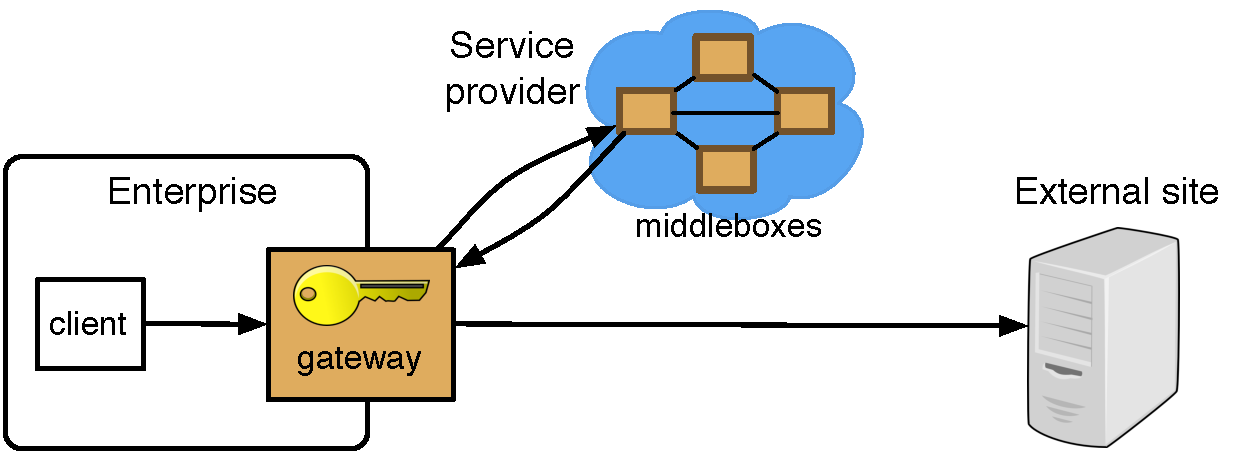
\includegraphics[width=3.3in]{fig/model_1.pdf}
  \label{fig:model1} }
%
\vfill  
\subfigure[Enterprise to enterprise communication]{
   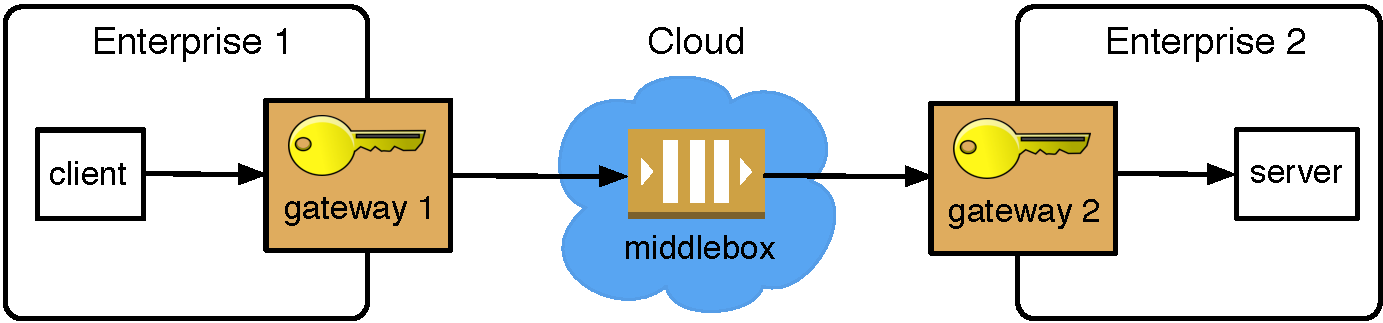
\includegraphics[width=3.1in]{fig/model_2.pdf}
     \label{fig:model2}}
%
\caption{System architecture: Aplomb and NEF system setup with \sys's encryption \label{fig:sys-overview}}
\end{figure}

\begin{itemize}
\item applications
\item use cases
\end{itemize}

\subsection{Threat model}

The goal of \sys is to protect the privacy of the traffic against an attacker at the cloud 
(cloud employee, or hacker gaining access to cloud machines). 
We consider a strong cloud attacker, one that has gained access to {\em all cloud data}.
This includes any traffic and communication the cloud receives from the 
gateway, any old logged information, cloud state, and so on. Nevertheless, we assume that 
the cloud provides good service and runs middlebox functionality correctly.  The concern is
about reading and leaking private data. 

We assume that the gateways are trusted. They do not leak information.


Some middlebox functionalities (such as intrusion detection, exfiltration detection) have a threat model
of their own about the client and the server. For example, intrusion detection assumes that 
the client or the server could misbehave and try to mount an attack, but at most one of them misbehaves 
(indeed, if both misbehave, they can send attack traffic to each other encrypted with a shared symmetric key and fundamentally
no one can detect such an attack).  We preserve all these threat models unchanged. These applications rely
on the good behavior of the middlebox to detect attacks in these threat models. Since we assume the middlebox executes
these functions correctly and \sys preserves the functionality of these middleboxes, 
these threat models are irrelevant to the protocols in \sys, and we will not discuss them again. 



\subsection{\sys overview}

To protect privacy of the traffic, \sys encrypts all traffic passing through the middlebox at the cloud. 
As in Fig.~\ref{fig:sys-overview}, the gateway has a secret key $k$; in the setup with two gateways, they share
the same secret key. The gateway encrypts all traffic going to the middlebox in the cloud using \sys's protocols.
The middlebox in the cloud processes {\em encrypted traffic} using \sys's protocols. 
After the processing, the middlebox
will produce encrypted traffic which it sends back to the gateway. The gateway decrypts the traffic using the key $k$, 
and forwards it as in the setup.

Throughout this process, MB handles only the encrypted traffic and never gets the decryption key. This ensures
that an attacker that steals all data from the cloud, will only see encrypted traffic and hence protects the privacy of the 
traffic. 

\sys encrypts IP addresses, ports, and the payload of the packet, thus protecting the privacy of all these parameters. 

At the same time, \sys supports a wide range of middlebox applications, in fact, all the applications considered in the 
Aplomb model.


\begin{table}[t!]
\begin{tabular}{p{3cm}|p{2cm}|p{1cm}}
Application  & Operations used & Details \\
\hline \hline
IP Firewall &    & \S\ref{sec:firewall} \\
Application Firewall &  & \S\ref{sec:firewall}\\
NAT &  & \S\ref{sec:nat} \\
IP Forwarding  & & \\
VPN Gateway &  none & \S\ref{sec:vpn} \\ 
Load Balancer L4 & & \S\ref{sec:loadb}\\
Load Balancer L7  & & \S\ref{sec:loadb}\\
WAN optimizer  &  & \S\ref{sec:not_supp}\\
Web proxy/cache  & & \S\ref{sec:proxy}\\
intrusion detection (IDS)  & & \S\ref{sec:IDS}\\
data exfiltration  & & \S\ref{sec:IDS} \\
\todo{split this} 
\end{tabular}
\caption{Middlebox applications supported by \sys. \label{tab:apps}}
\end{table}



\todo{need to discuss what happens to SSL connections here; what if the client initiates one? the gateway can no longer
encrypt things}

- security guarantees


-- handling two gateways with non-determinism




-- goals on the gateway

-- have a way to show that what the gateway does is generic 
   
-- somewhere we need to discuss goals regarding the gateway

-- why we choose certain operations

which app for which operation


- need to discuss somewhere the above goals from the gateway
%A LOT OF SYSTEMS BUILDING


- why we choose certain operations

